\chapter{Introduction to U.S. International Taxation}

\intro{This chapter briefly overviews the U.S. international tax system.  It describes the concepts of residence and source basis taxation, the basic U.S. tax rules applicable to foreign person with U.S. activities and U.S. persons with foreign activities, and the role and function of income tax treaties.}
		
International tax refers, in this book, to the set of U.S. tax rules that apply to foreign persons investing or transacting business in the United States and U.S. persons investing or engaging in business outside of the United States.  Some examples of where these rules apply include:  the payment of interest or dividends by a U.S. corporation to a foreigner; the temporary assignment of a foreign executive to the United States; the U.S. branch operations of a foreign bank; a U.S. attorney working in London; the establishment of an Asian manufacturing and distribution network by a U.S. corporation; the sales of cars by Toyota Japan to its U.S. subsidiary; and the transfer by a U.S. corporation of intellectual property to an offshore affiliate to be used in producing property to be sold.  The rules governing these transactions are found in the Internal Revenue Code and accompanying Treasury regulations; administrative guidance, such as revenue rulings; judicial decisions; and bi-lateral tax treaties between the United States and its major trading partners.  

If no one in the U.S. invested abroad or no foreigner invested in United States, there would be no need for this special tax regime.  Very fortunately, that is not the universe we inhabit for it would be a poor and miserable one.  A quick flip through the history books or a few minutes reading about the economic fortunes of residents of countries closed to international trade and investment, \textit{e.g.}, North Korea at beginning of the 21st century, should quickly disabuse anyone of the notion that an economy closed to foreigners and their capital is one in which you would like to live, work or raise a family.  Also, for those in whom xenophobic tendencies rage strong, don't hold your breath that cross-border investment or trade will cease anytime in the near future:  the continuing U.S. trade deficits--exports minus imports--ensures that foreigners will have excess dollars that need to be invested in U.S. assets.  The following chart displays the significant growth in both inbound and outbound direct investment over the  last 33 years.

 \begin{figure}[hbtp]
 \caption{Inbound and Outbound Direct Investment}
 \begin{center}
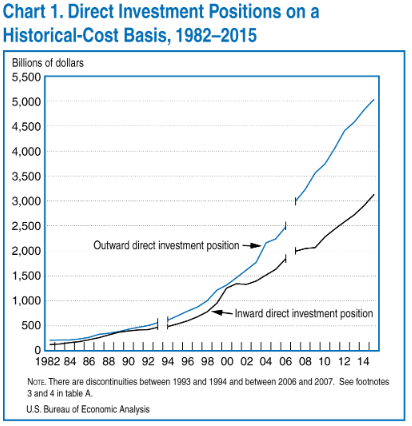
\includegraphics[width=110mm, height=80mm,clip, trim= 3mm 4mm 4mm 20mm]{DirectInvest_2015.png}
% \setlength\fboxsep{0pt}
 %\setlength\fboxrule{0.5pt}
 %\fbox{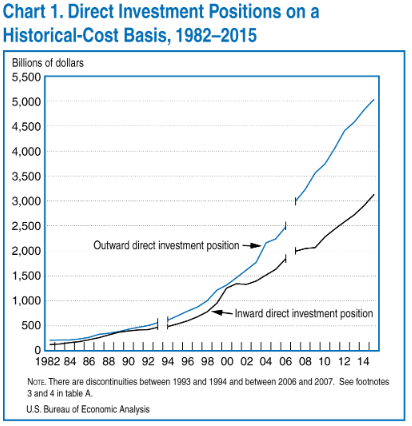
\includegraphics[width=120mm, height=75mm, clip, trim= 5mm 8mm 5mm 20mm]{DirectInvest_2015.png}}
 \end{center}
 \label{your-reference-key}
 \end{figure} 

The U.S. international tax rules are found primarily in subchapter N (sections 861 through 999) of the Internal Revenue Code, but scattered outside of subchapter N are some important international tax provisions, such as section 367 (reorganizations involving foreign corporations), section 482 (related party transactions), section 1248 (sales of the stock of foreign corporations), and sections 1291-1298 (passive foreign investment companies).  Importantly, the principles and rules you have learned in your other tax classes regarding the timing of an item of income or deduction, the tax classification (interest, dividend, or sale of goods or services), and the tax character (ordinary income or capital gain), do not cease to apply because one of the parties is foreign or the transaction occurs abroad.  In fact, because many types of income earned by foreigners, such as capital gains, are generally exempt from U.S. tax, these determinations are often more important for foreigners than domestic taxpayers.

%but The primary reason is the continued importance of cross-border trade and investment.  As U.S. individuals and firms venture outside of the United States to sell their labor, to manufacture and sell products, license their intangible property or invest their capital, the country in which these activities occur may tax the wages, revenues, royalties, or investment returns generated by these activities.  The United States may also tax those same returns. Foreign individuals and firms face similar tax issues when they carry on economic activities in the United States. 

							%Here: data on cross border trade and investment
							%Technical Considerations : Code /regs, etc
							% Important considerations:  affect investment choice and structure, pricing assets
	\section{Overview  Source and Residence Basis Taxation}
	
Most countries \margit{Source basis taxation applies to income arising in a country.} exert their taxing authority on two bases or types of jurisdictions: source and residence.  A country exercises \emph{source basis} tax jurisdiction over income arising within its borders that is earned by a foreign person, which can be an individual, corporate entity, or sovereign.  A dividend paid by a U.S. corporation, for example, is classified as U.S. source income, and if received by a foreign person, is generally subject to U.S. tax, even though the foreign person was never physically present in the United States.  The rationale behind source basis taxation is that the source country has provided the primary benefits, such as infrastructure, markets, and property rights,  to generate the income.    
	
Two distinct \margit{Foreign persons are taxed on a \emph{gross} basis on U.S. source investment income and on a net basis on U.S. source business income.} U.S. tax regimes apply to U.S. source income earned by foreign persons.  Foreign persons who earn only U.S. source passive or investment income such as dividends, rents, and royalties, are taxed at a flat 30\% rate (no deductions permitted).  In contrast, foreign persons who have a U.S. trade or business are taxed on the \emph{net}  U.S. source income (gross income reduced by allocable deductions) that is ``effectively connected'' with the U.S. trade or business at the same graduated rates applicable to U.S. persons. Gains from the sale of U.S. real property interests are taxed as effectively connected income. 

A country exerts \emph{residence basis} taxation \margit{Residence basis taxation applies to persons, including legal persons.} over persons on the basis of their legal status.  Persons (including legal persons such as corporations) subject to residence basis taxation are taxed on their worldwide income.  Under the ability-to-pay principle, residence basis taxation is justified on the grounds that both U.S. and foreign source income equally affect a person's ability to pay.  In addition, exempting foreign source could cause capital to flow abroad even if it could be more profitably invested in the United States.

The United States taxes its citizens, resident aliens, and corporations incorporated in one of the fifty states on a residence basis.  The United States, it should be noted, is unique among economically advanced nations in taxing its nonresident citizens on a residence basis and the foreign business income of its corporations. 

A U.S. person could easily avoid U.S. residence basis taxation merely by forming a foreign corporation and holding investment and business assets in the corporation.  Left unchecked, such a system could lead to a substantial reduction in U.S. tax revenue and an uneconomic skewing of investment and business capital.  To thwart such tax planning, the U.S. has enacted two anti-deferral regimes, the controlled foreign corporation and the passive foreign investment company regimes, under which U.S. shareholders of these foreign corporations are taxed currently on some or all of the corporations' current earnings regardless of whether the earnings are actually distributed to the shareholders (or are subject to an interest charge when the earnings are distributed).  Importantly, however, the business income of a controlled foreign corporation is generally not taxed by the United Sates until the income is remitted to the corporation's U.S. shareholder, typically the U.S. parent.  

The treatment of business profits earned by foreign subsidiaries of U.S.-based multinational corporations presents many policy and administrative challenges.  Some argue that such profits should be taxed currently at regular corporate rates (or a reduced rate) so that U.S. multinationals will not have a tax incentive to locate operations and jobs offshore.  Others argue that since most other developed countries do not tax the foreign business operations of their multinationals, if the United States taxed the offshore operations of its multinationals, the U.S. multinationals would be at a competitive tax disadvantage vis-a-vis their foreign counterparts.  

In recent years, U.S. multinationals and their foreign competitors have developed sophisticated tax structures that reduce and often eliminate any source basis taxation on business profits, leading to the rise of so-called \emph{stateless income}.  This development has caused much consternation among developed countries as their tax administrators see a marked drop in business tax revenues.  

In an effort to avoid the sting of the U.S. anti-deferral regimes, some U.S. multinationals have  \textit{inverted} their corporate structure by making the former U.S. parent a subsidiary of a new foreign parent, but without changing the identity of the shareholders.  Also, some recent public mergers between U.S. and foreign companies have resulted in inverted structures as well, much to the chagrin of some members of Congress and U.S. tax administrators.  Although there are U.S. tax provisions that attempt to discourage inversions, many commentators believe that they need to be strengthened.       

International double taxation arises when two or more countries assert tax jurisdiction over the same income or same persons.  For example, if a U.S. resident receives a dividend from a U.K. corporation and the U.K taxes the dividend, the dividend will be taxed twice, once by the United States on a residence basis and once by the United Kingdom on a source basis.   Double taxation is anathema to both taxpayers and governments: multiple layers of taxation can quickly become confiscatory, and if left unchecked, would significantly reduce cross-border trade and investment.  

To ameliorate double taxation, \margit{Double taxation is generally mitigated by the residence country ceding primary tax jurisdiction to the source country.   Source trumps residence.}the residence country generally cedes taxing primary jurisdiction to the source country.  The justification is that the source country is primarily responsible for the generation of the income, and source basis taxation should therefore take precedence. The United States unilaterally mitigates double taxation by allowing a credit for foreign taxes paid on foreign source income.  Other countries mitigate double taxation through a credit system, exemption of foreign source income, or a particular tax treaty provision.  Even if every country had the same double tax relief mechanism, however, double taxation would invariably arise because of different national definitions of residence, source, and the characterization of income.  

	\section{Overview of Income Tax Treaties}
	
To resolve these fundamental fiscal conflicts, countries enter into bi-lateral income tax treaties.  Treaties, which generally take precedence over domestic law, mitigate double taxation by providing rules of precedence when fiscal conflicts arise.  For example, a person who is a resident of more than one country--a U.S. green card holder residing in another country--could be subject to residence basis taxation by both the United States and his country of residence.  Tax treaties prevent this by establishing a single fiscal residence.  Treaties also often contain specific source rules and double tax relief provisions, the latter being especially important for persons residing in a country without a domestic foreign tax credit.   

Treaties \margit{Treaties lower source basis taxation and thereby increase the revenue of residence countries.}also aim to foster increased trade and investment by lowering source country taxation.  U.S. source dividends paid to a foreign treaty resident, for instance, are generally taxed at a maximum 15\% (or sometimes 5\% or 0\%) instead of 30\% under U.S. domestic law.  Also, income of a U.S. trade or business earned by a treaty resident is not taxed by U.S. unless the trade or business rises to the level of a \textit{permanent establishment}, which requires more substantive activities and presence than a trade or business.  By lowering source basis taxation, treaties in essence shift tax revenue from source countries to residence countries.  

Most tax treaties are based on the Organization of Economic Cooperation and Development (OECD) Model Tax Convention on Income and Capital and the detailed Commentaries, which are used in implementing and interpreting treaty provisions.  The OECD Model Treaty was first developed in 1958 and was based on the work of economists from the 1920's.\footnote{ The OECD was  formed in 1960 when 20 countries (the 18 members of the Organization for European Economic Cooperation, the United States, and Canada)  signed the OECD Convention, which endeavors to promote growth and improved standards of living for members, sound economic expansion of member countries, and expansion of world trade.  Since its founding the OECD has grown to include 34 members from around the world, with Chile, Estonia, Israel, and Slovenia becoming the most recent countries to join.}  

The United States has entered into over 60 income tax treaties, including treaties with almost all of its major trading and investment partners, and is continually expanding its treaty network.  The United States also has issued various model treaties, the most recent being the 2016 U.S. Model Treaty, which supersedes the 2006 Model.  The technical explanation is expected to be issued in 2017.  The model treaties are updated to reflect changes in U.S. tax policy.   

This book uses the U.S.-U.K.income tax treaty as its reference treaty. This treaty was signed in 2001 and came into force on March 31, 2003.  The U.S.-U.K. treaty is a treaty with a major trading partner and contains many provisions that specifically reflect recent U.S. international tax policy concerns.  The U.S.-U.K. treaty and the U.S. Treasury Technical Explanation of the Treaty are found in Appendix A.  I opted to use an actual tax treaty rather than either the OECD or U.S. Model Treaty mostly to avoid awkward phrasings such as ``X is a resident of a country with which the U.S. has tax treaty identical to the U.S. or OECD Model Treaty,'' or ``X is a resident of Treatyland.''  In addition, you can see how a particular treaty resolves specific conflicts that arise when two separate fiscal regimes meet.    

This rise of stateless income and the concern that unilateral responses by OECD members could result in double taxation  and increased tax uncertainty for cross-border investments led the OECD to address base erosion and profit shifting in the context of cross-border transactions.  In response to their findings, the OECD approved in 2013 the \emph{BEPS Action Plan}, which identified 15 action items that required new international standards.\footnote{OECD, Action Plan on Base Erosion and Profit Shifting, July 19, 2013, available at \url{http://www.oecd.org/tax/action-plan-on-base-erosion-and-profit-shifting-9789264202719-en.htm}}  Key action items were electronic commerce, hybrid mismatch arrangements, transfer pricing aspects of intellectual property, CFC rules, interest deductibility, and data collection.  Final reports on all items were finished in 2015 and endorsed by the G20 leaders.  Individual countries, including the United States, have already begun to implement some of the action items.\footnote{Recent developements and country-by-country trackers can be found in at the following links:   \url{http://www2.deloitte.com/global/en/pages/tax/articles/beps-country-scorecards.html}; \url{http://www.ey.com/GL/en/Services/Tax/OECD-base-erosion-and-profit-shifting-project} } We'll visit many of these topics throughout the semester.

 

\section{Overview of Text}
After examining the rules that classify persons as foreign or U.S. and legal entities as either partnerships or corporations, we will focus our study of U.S. international tax rules on two main areas: (1) \margit{\emph{Inbound} refers to the taxation of foreigners' U.S. investments and activities, and \emph{Outbound} to the taxation of the foreign operations of U.S. persons} the taxation of foreigners investing and doing business in the United States (source basis tax jurisdiction); and (2) the taxation of U.S. persons investing and doing business abroad (residence basis jurisdiction), including the U.S. anti-deferral regimes, \emph{i.e.}, the controlled foreign corporation and passive foreign investment provisions, and the foreign tax credit regime, the domestic mechanism the United States employs to coordinate overlapping tax jurisdiction.  Tax treaty provisions are integrated throughout with the relevant domestic provisions.  We also examine section 482, which requires related parties to deal with each other on an arm's-length basis.  This important provisions applies to both U.S. and foreign taxpayers.  

Along the way, we will also examine some proposals to modify the current U.S. international tax regime, as Congress and Treasury grapple on one hand with concerns of U.S.-based multinationals that the U.S. tax system places them at a competitive disadvantage vis-a-vis their foreign competitors and on the other that our current tax system favors foreign investment over U.S. investment thus encouraging jobs and capital to move oversees.  It is virtually certain that we'll see in 2017 some of the most signficant changes to the U.S. international tax regime in the last 50 years.  

Like other parts of the Internal Revenue Code, the international tax provisions reflect many compromises among competing objectives such as fairness vis-a-vis U.S. taxpayers, revenue raising, administration, and encouraging foreign investment. Because these objectives are sometimes contradictory, the U.S. international tax rules are not entirely consistent or simple.  But that makes the course stimulating and challenging and the field an interesting and potentially lucrative one to work in.  

	\begin{framed}
		Last revised:  Jan. 10, '17
			\end{framed}

 